\section{Identification}
\label{sec:ident}

The identification module contains structures and methods for the identification of model images and contains the following sub-modules:

\begin{description}

\item[Photoframe identification]~: Module with structures and methods for texture identification using a photoframe around the model image.
\item[Texture identification]~: Module with structures and methods for texture identification. This module allows the user to define textured model images. The identification at run-time is generally slower than the database identification but can be accelerated using a photoframe around the model image.
\item[Database identification]~: Module with structures and methods for model identification in a database.The database identification module needs the generation of a database from an image model. This offline generation step is time consuming but can be performed once and for all. At runtime, the database identification is faster than the texture identification since many computations have already been done offline.
\end{description}

\subsection{Photoframe identification}
\label{sse:ident_photoframe}

\noindent The photoframe identification module performs the identification of textured model images with a black frame around the texture as shown in Figure~\ref{fig:ident_photoframe}. 

\begin{figure}[H]
\centering
\includegraphics[width=0.45\textwidth]{vision/figures/ident_photoframe} 
\caption{Examples of model that can be identified with the photoframe identification module.}
\label{fig:ident_photoframe}
\end{figure}

The photoframe image model identification is faster than the
identification of phototexture image model since the identification
take benefit of the detection of the black frame around the texture.
On the other hand, the black frame shall be fully visible in the image.

\subsubsection{The {\tt Rox\_Ident\_Photoframe\_SE3} object}
\label{sss:ident_photoframe_object}
A \lstinline$Rox_Ident_Photoframe_SE3$ object is a pointer to the opaque structure \lstinline$Rox_Ident_Photoframe_SE3_Struct$: 

\begin{lstlisting}
typedef struct Rox_Ident_Photoframe_SE3_Struct * Rox_Ident_Photoframe_SE3
\end{lstlisting}

\subsubsection{Creating/Deleting a {\tt Rox\_Ident\_Photoframe\_SE3}}
\label{sss:ident_photoframe_newdel}
~\\

\noindent The rox\_ident\_photoframe object shall be created before any call to other functions using it :

\begin{lstlisting}
Rox_Error rox_ident_photoframe_new(Rox_Ident_Photoframe * ident_photoframe) 
\end{lstlisting}

\noindent This function creates a new empty database object.

\begin{lstlisting}
Rox_Error rox_ident_photoframe_del(Rox_Ident_Photoframe * ident_photoframe)
\end{lstlisting}


\subsubsection{Main functions related to {\tt Rox\_Ident\_Photoframe\_SE3}}
\label{sss:ident_photoframe_functions}
~\\

\noindent A photoframe is a planar object specifically designed to be identified
when filmed with a camera. It is a composition of an image template, a
thick black border and a white background outside of the border.
Figure 1 explains the common scheme of a photoframe.  The image inside
the black borders is the \emph{template}. This template is the object
to identify, and which will be used to track the object after
detection if needed. This template size is
$\left[image \; rows, image \; cols\right]$.  Values iheight and iwidth shall be
equal to 128 pixels.

\begin{figure}[h]
\centering{}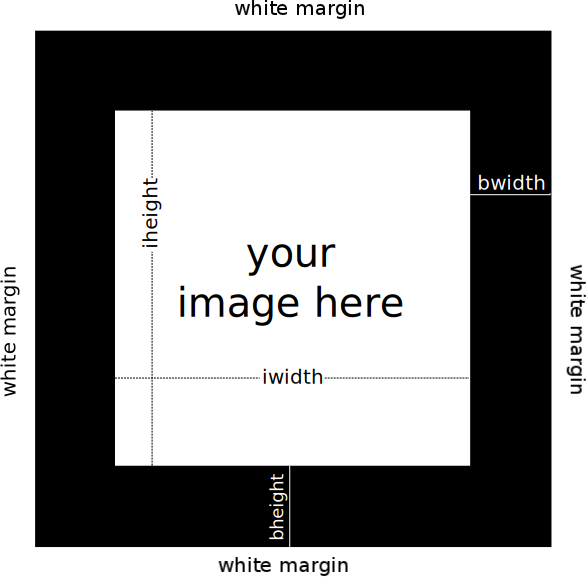
\includegraphics[width=0.6\columnwidth]{vision/figures/fake}
\caption{A common photoframe scheme}
\end{figure}

\noindent The border size $\left[border \; rows, border \;
  cols\right]$ is choosed optimally to be visible in a large set of
viewpoints while not being too large (i.e. not wasting image space).
The following calculus is done to compute border size :

\begin{itemize}
\item border rows = $\frac{80}{512}$ image rows
\item border cols = $\frac{80}{512}$ image cols
\end{itemize}

\noindent Be sure to respect those sizes when creating your photoframe or the
identification performance will be severely degraded.\\

\noindent To create a photoframe, choose a template image which is compatible
with \rox{} (non uniform, with enough texture). Store this template in
a PGM image file. With an image editing software (E.g. : photoshop,
gimp) draw the borders in black color (See figure 1). Print this image
on a white paper sheet. Because of printers approximation, it is not
possible to know what will be the exact size (in meters) of this
print.  Take a ruler to measure the width and height of the image
template \emph{inside} the black borders. These real sizes are only
needed if used to compute odometry after identification. Repeat this
operation for each photoframe you need.\\

\noindent The user can go through the following workflow:

\begin{enumerate}
\item An identification structure is created (see section~\ref{sss:ident_photoframe_newdel}).
\item Template images are added to the identification module using the following function:

\begin{lstlisting}
Rox_Error 	rox_ident_photoframe_se3_addframe (Rox_Ident_PhotoFrame_SE3 obj, Rox_Image model, Rox_Real width_meter, Rox_Real height_meter, Rox_Uint border_width);
\end{lstlisting}

\noindent Adds a new template to a photoframe identification
structure. Shall be called before identification. First parameter is a
pointer created with rox\_ident\_new, second parameter is the template
image to add (without black borders) with a size of 128x128 pixels.
Please note that one photoframe will be identified only once in one
image. If several instances of the same photoframe are in the
processed image, only the first found will be considered. Note that
the identifier of the added photoframe will be the number of times
this function has already been called.

\item The user grabs an image from a stream (e.g. a camera) and gives it
  to photoframe identification. The identification is done and the
  number of identified templates are stored in the \lstinline $Rox_Ident_PhotoFrame_SE3$ object:

\begin{lstlisting}
Rox_Error rox_ident_photoframe_se3_make (Rox_Ident_PhotoFrame_SE3 obj, Rox_Camera camera);
\end{lstlisting}

\noindent Using the ident structure created with rox\_ident\_new and filled
with templates using rox\_ident\_add\_photoframe, tries to detect
photoframes in the given image. This image may be given by a camera
for example. Returns the number of identified photoframes in the current
image.

\item For each template, the user can check if it has been identified using the following function:

\begin{lstlisting}
Rox_Error rox_ident_photoframe_se3_getresult (Rox_Uint *is_identified, Rox_MatSE3 pose, Rox_Ident_PhotoFrame_SE3 obj, Rox_Uint id);
\end{lstlisting}

\noindent Used after a call to rox\_ident\_photoframe. Checks if a given photoframe
(using its id) has been detected or not. ident is a
pointer to a photoframe identification structure created with rox\_ident\_new.
photoframe\_id is a number between 0 and the number of added frames.
Returns Rox\_True if the specific photoframe is detected, Rox\_False
otherwise.

% \item If the template is identified, a function returns a 2D transformation which
% measures how the template is ``seen'' in the current grabbed image.

% \begin{lstlisting}
% Rox_MatSL3 rox_ident_photoframe_get_matsl3(Rox_Ident ident, Rox_Uint id);
% \end{lstlisting}

\noindent Used after a call to rox\_ident\_photoframe and rox\_ident\_get\_identified.
If a photoframe with id has been identified, returns the 2D
transformation which represents the template image (without the borders)
in the current image. 2D transformation is not defined (and may contain
random value) if the marker is not identified.\\

\item Once not used anymore, the identification structure shall
be deleted (see section~\ref{sss:ident_photoframe_newdel}).
\end{enumerate}

\subsection{Texture identification}
\label{sse:ident_texture}

\noindent The texture identification module performs the identification of textured model images as shown in Figure~\ref{fig:ident_texture}. 

\begin{figure}[H]
\centering
\includegraphics[width=0.45\textwidth]{vision/figures/ident_phototexture} 
\caption{Example of image model that can be identified with the texture identification module.}
\label{fig:ident_texture}
\end{figure}

\subsubsection{The {\tt Rox\_Ident\_Texture\_SE3} object}
\label{sss:ident_texture_object}
A \lstinline$Rox_Ident_Texture_SE3$ object is a pointer to the opaque structure \lstinline$Rox_Ident_Texture_SE3_Struct$: 

\begin{lstlisting}
typedef struct Rox_Ident_Texture_SE3_Struct * Rox_Ident_Texture_SE3
\end{lstlisting}


\subsubsection{Creating/Deleting a {\tt Rox\_Ident\_Texture\_SE3}}
\label{sss:ident_texture_newdel}

\noindent Functions are provided to allocate and deallocate a \lstinline$Rox_Ident_Texture_SE3$ object~:

\begin{lstlisting}
Rox_Error rox_ident_texture_se3_new (Rox_Ident_Texture_SE3 *ident_texture);
\end{lstlisting}

\noindent The function creates a new identification structure. Shall be called before
any other function of this module. Returns a pointer to the Rox\_Ident\_Texture object. \\

\begin{lstlisting}
Rox_Error 	rox_ident_texture_se3_del (Rox_Ident_Texture_SE3 *ident_texture); 
\end{lstlisting}

\noindent Deletes an identification structure. First parameter is a pointer
created with rox\_ident\_texture\_new. Shall be called to free up memory when
user does not need identification anymore.

\subsubsection{Main functions related to {\tt Rox\_Ident\_Texture\_SE3}}
\label{sss:ident_texture_functions}
~\\

A model to be identified can be set using the following function:
\begin{lstlisting}
Rox_Error rox_ident_texture_se3_set_model (Rox_Ident_Texture_SE3 ident_texture, Rox_Model_Single_Plane model); 
\end{lstlisting}
A function is available to identify a given model in a camera object: 
The second function input the camera containing the current image in which to identify the texture:
\begin{lstlisting}
Rox_Error rox_ident_texture_se3_make (Rox_MatSE3 pose, Rox_Ident_Texture_SE3 ident_texture, Rox_Camera camera);
\end{lstlisting}

% If identification is successfull, the resulting homography matrix locating the serched texture in the image can be obtained with the following function: 
% \begin{lstlisting}
% Rox_Bool rox_ident_texture_get_matsl3_copy(Rox_MatSL3 H, Rox_Ident_Texture ident_texture)
% \end{lstlisting}

%\begin{lstlisting}
%Rox_MatSL3 rox_ident_texture_get_matsl3(Rox_Ident_Texture ident_texture) 	
%\end{lstlisting}

\subsection{Database identification}
\label{sse:database}

The computation of visual information (e.g. keypoints features) needed
for image identification can be done offline and stored in a database.
For each image model we would like to identify in the current image, a
specific database item is created. Several items can also mixed
together to allow the identification of multiple images.

Figure~\ref{fig:ident_database} illustrates the structure of the database identification module:

\begin{figure}[H]
\centering
\includegraphics[width=0.75\textwidth]{vision/figures/ident_database} 
\caption{Structure of the database identification module.}
\label{fig:ident_database}
\end{figure}

\subsubsection{The {\tt Rox\_Ident\_Database\_SE3} object}
A \lstinline$Rox_Ident_Database_SE3$ object is a pointer to the opaque structure \lstinline$Rox_Ident_Database_SE3_Struct$: 

\begin{lstlisting}
typedef struct Rox_Ident_Database_SE3_Struct * Rox_Ident_Database_SE3
\end{lstlisting}

\subsubsection{Creating/Deleting a {\tt Rox\_Ident\_Database\_SE3}}

\noindent One database item is associated to one template. A Rox\_Ident\_Database may be considered as a collection of such database items. The database identification module is able to identify several templates simultaneously. Current library is optimized to run on up to 150 simultaneous templates. User can ask the module to detect all possible templates in the same current image or to detect only the most visible template (among the templates in the database). Speed degrades with the number of templates to track simultaneously and quality degrades with the number of templates in the database. It is possible to create several Rox\_Ident\_Database objects in the same program.\\

\noindent The rox\_ident\_database object shall be created before any call to other functions using it :

\begin{lstlisting}
Rox_Error rox_ident_database_se3_new (Rox_Ident_Database_SE3 *ident, Rox_Uint max_templates_simultaneous);
\end{lstlisting}

\noindent This function creates a new empty database object.

\begin{lstlisting}
Rox_Error rox_ident_database_se3_del (Rox_Ident_Database_SE3 *ident);
\end{lstlisting}

This function deletes the object. Shall be called when you do not need this database object anymore.

\subsubsection{Main functions related to {\tt Rox\_Ident\_Database\_SE3}}

% \begin{lstlisting}
% Rox_Bool rox_ident_database_add_template(Rox_Ident_Database
% obj, Rox_Char * pathtodb, Rox_Uint template_height, Rox_Uint template_width)
% \end{lstlisting}

% \noindent This function adds a template database file to the Rox\_Ident\_Database object. Please take care not to add several times the same database file. Template dimensions (template\_height and template\_width) are the dimensions of
% the reduced image to be used for further tracking process. Each time you add a
% template, an internal counter is incremented. The value of this counter is used
% as a unique ID for this template. Thus the template ID is a number between
% 0 and N-1 (N being the number of added templates).

\noindent The following function shall be called to enable
identification and prepare internal structures for optimized
execution:
\begin{lstlisting}
Rox_Error rox_ident_database_se3_set_database (Rox_Ident_Database_SE3 ident, Rox_Database db);
\end{lstlisting}

\noindent The following function execute identification process on the
image contained in the camera object. Uses all the templates added and
compiled before the call to this function. Once a template is found,
an internal flag is set and it will be ignored in further calls to
rox\_ident\_database\_process.
\begin{lstlisting}
Rox_Error rox_ident_database_se3_make (Rox_Ident_Database_SE3 ident, Rox_Camera camera);
\end{lstlisting}

\noindent To get the identification result for a given template ID use the following function: 

\begin{lstlisting}
Rox_Error rox_ident_database_se3_getresult (Rox_Uint *is_identified, Rox_MatSE3 pose, Rox_Ident_Database_SE3 ident, Rox_Uint id); 
\end{lstlisting}

\subsubsection{Creation of database items}

\noindent First, retrieve an image of your template without any perspective distortion. The biggest the image is, the better the detection will perform after database creation. However, if the image is too big the database file will be large and long to create. Ideally, the template size should be close to the image that will be viewed by the camera. The template image shall not contain large textureless regions and shall contain visual information everywhere. Please keep both files in a directory as they will be necessary for identification process.

The programmer can create its own database items by using the following function:
\begin{lstlisting}
Rox_Error rox_database_item_learn_template (Rox_Database_Item item, Rox_Image template); 
\end{lstlisting}

A database item can be saved on disk (use the extension ``.rdi'' for database items) using the following function:
\begin{lstlisting}
Rox_Error rox_database_item_save (Rox_Char *filename, Rox_Database_Item item);
\end{lstlisting}
A database item can be loaded using the following function:
\begin{lstlisting}
Rox_Error rox_database_item_load (Rox_Database_Item item, Rox_Char *filename);
\end{lstlisting}

%The programmer can create its own database item (extension .rdb) by using the following function:
%\begin{lstlisting}
%Rox_Bool rox_ident_database_create(const char *rdb_filename, Rox_Image image)
%\end{lstlisting}

\subsubsection{Creation of a database}

\noindent A database object shall be created using the following function:

\begin{lstlisting}
Rox_Error rox_database_new (Rox_Database *db));
\end{lstlisting}

\noindent This function creates a new empty database object.

The following function deletes the object.

\begin{lstlisting}
Rox_Error rox_database_del (Rox_Database *db); 
\end{lstlisting}
Shall be called when you do not need this database object anymore.

A database item can be added to the database using the following function:

\begin{lstlisting}
Rox_Error rox_database_add_item (Rox_Database database, Rox_Database_Item item, Rox_Real sizx, Rox_Real sizy);
\end{lstlisting}

After adding several items to the database, they can be fused in the database using the following function:

\begin{lstlisting}
Rox_Error rox_database_compile (Rox_Database database);
\end{lstlisting}

The resulting database can be saved on disk (use the extension ``.rdb'' for databases) using the following function:

\begin{lstlisting}
Rox_Error rox_database_save (char *filename, Rox_Database database);
\end{lstlisting}

and loaded from disk using the following function:

\begin{lstlisting}
Rox_Error rox_database_load (Rox_Database db, char *filename);
\end{lstlisting}

For client/server applications the user can serialise a database using the following function:
\begin{lstlisting}
Rox_Error rox_database_serialize (char *buffer, Rox_Database db);
\end{lstlisting}
and after sending it through the network, the user can deserialise it using the following function:
\begin{lstlisting}
Rox_Error rox_database_deserialize (Rox_Database db, char *buffer);
\end{lstlisting}

\subsubsection{Identification using database features directly}

In some applications, like cloud client/server applications, it is useful to store and use directly database features for the identifications. The features are stored in a Rox\_Database\_Features object. 

The programmer can use the following function to create database features:
\begin{lstlisting}
Rox_Error rox_database_features_new (Rox_Database_Features *features);
\end{lstlisting}

The Rox\_Database\_Features object can be deleted using the following function:
\begin{lstlisting}
Rox_Error rox_database_features_del (Rox_Database_Features *features);
\end{lstlisting}

The reference image can be therefore identified using the database features:
\begin{lstlisting}
Rox_Error rox_ident_database_se3_make_features (Rox_Ident_Database_SE3 ident, Rox_Database_Features features, Rox_Matrix calib_camera);
\end{lstlisting}


In the first case, the programmer can also serialize/deserialize the information in the Rox\_Database\_Features object in order to be sent through a network socket: 
\begin{lstlisting}
Rox_Error rox_database_features_serialize (Rox_Char *buffer, Rox_Database_Features features);
\end{lstlisting}

\begin{lstlisting}
Rox_Error rox_database_features_deserialize (Rox_Database_Features features, Rox_Char *buffer);
\end{lstlisting}

In the second case, the file containing the database features can be
created using the following function:
\begin{lstlisting}
Rox_Error rox_database_features_save (Rox_Char *filename, Rox_Database_Features features);
\end{lstlisting}
The file can be loaded using the following function:
\begin{lstlisting}
Rox_Error rox_database_features_load (Rox_Database_Features features, Rox_Char *filename);
\end{lstlisting}

See the example ``rox\_example\_identification\_database\_cloud.c'' for an example of use.

%\subsection{Offline identification}
\label{sse:ident_offline}

\noindent The offline identification module performs the identification of textured model images similarly to the texture identification module. However, higher precision and rate of success are targeted. Thus, the offline identification module is generally much slower than the texture identification module and should be used for offline applications.

\subsubsection{Creating/Deleting a {\tt Rox\_Ident}}
\label{sss:ident_newdel}
~\\

\noindent Functions are provided to allocate and deallocate a \lstinline$Rox_Ident$ object~:

\begin{lstlisting}
Rox_Image rox_ident_new(Rox_Void);
\end{lstlisting}

\noindent The \lstinline$rox_ident_new$ creates a new identification structure. Shall be called before
any other function of this module. Returns a Rox\_Ident pointer. \\

\begin{lstlisting}
Rox_Void rox_ident_del(Rox_Ident ident);
\end{lstlisting}

\noindent Deletes an identification structure. First parameter is a pointer
created with rox\_ident\_new. Shall be called to free up memory when
user does not need identification anymore.

\subsubsection{Main functions related to {\tt Rox\_Ident}}
\label{sss:ident_functions}
~\\

\noindent The following functions can be used for the identification of a planar textured object:

\begin{lstlisting}
Rox_Void rox_ident_set_method(Rox_Ident ident, const Rox_Uint method);
\end{lstlisting}

\noindent Set the identication method:
\begin{itemize}
\item method = 2 : fast identification method but less robust
\item method = 1 : slow identification method but more robust
\item method = 0 : total (try both fast and slow identification methods)
\end{itemize}
The default identification method is 0.

\begin{lstlisting}
Rox_Bool rox_ident_make(Rox_Ident ident, Rox_Image image_model, Rox_Image image_search);
\end{lstlisting}

\noindent Identify the image image\_model into the current image image\_search. Return ROX\_TRUE if the image\_model is identified in the image\_search.

\begin{lstlisting}
Rox_Void rox_ident_get_matsl3_copy(Rox_MatSL3 H, Rox_Ident ident);
\end{lstlisting}

\noindent Get the homographhy matrix H allowing to transform the corners if the model image into the corresponding corners in the image\_search.

